%; whizzy chapter
% -initex iniptex -latex platex -format platex -bibtex jbibtex -fmt fmt
% $B0J>e(B whizzytex $B$r;HMQ$9$k>l9g$N@_Dj!#(B

%     Kansai Debian Meeting resources
%     Copyright (C) 2007 Takaya Yamashita
%     Thank you for Tokyo Debian Meeting resources

%     This program is free software; you can redistribute it and/or modify
%     it under the terms of the GNU General Public License as published by
%     the Free Software Foundation; either version 2 of the License, or
%     (at your option) any later version.

%     This program is distributed in the hope that it will be useful,
%     but WITHOUT ANY WARRANTY; without even the implied warranty of
%     MERCHANTABILITY or FITNESS FOR A PARTICULAR PURPOSE.  See the
%     GNU General Public License for more details.

%     You should have received a copy of the GNU General Public License
%     along with this program; if not, write to the Free Software
%     Foundation, Inc., 51 Franklin St, Fifth Floor, Boston, MA  02110-1301 USA

%  preview (shell-command (concat "evince " (replace-regexp-in-string "tex$" "pdf"(buffer-file-name)) "&"))
% $B2hA|%U%!%$%k$r=hM}$9$k$?$a$K$O(Bebb$B$rMxMQ$7$F(Bboundingbox$B$r:n@.!#(B
%(shell-command "cd image200708; ebb *.png")

%%$B$3$3$+$i%X%C%@3+;O!#(B

\documentclass[mingoth,a4paper]{jsarticle}
\usepackage{kansaimonthlyreport}
\usepackage[dvips]{xy}
\usepackage{ascmac}

% $BF|IU$rDj5A$9$k!"Kh7nJQ$o$j$^$9!#(B
\newcommand{\debmtgyear}{2010}
\newcommand{\debmtgdate}{22}
\newcommand{\debmtgmonth}{08}
\newcommand{\debmtgnumber}{38}

\begin{document}

\begin{titlepage}

% $BKh7nJQ99$9$kItJ,!"K\J8$NKvHx$b=$@5$9$k$3$H$r$o$9$l$:$K(B

 $BBh(B\debmtgnumber{}$B2s(B $B4X@>(B Debian $BJY6/2q;qNA(B

\vspace{2cm}

\begin{center}
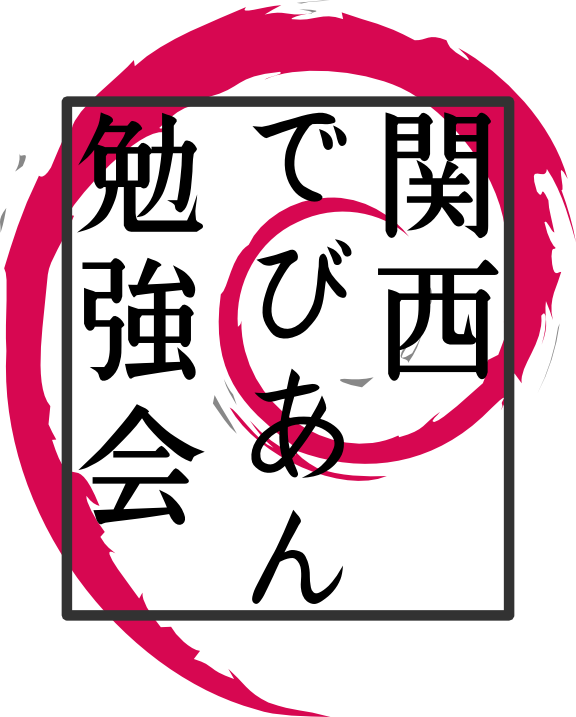
\includegraphics{image200802/kansaidebianlogo.png}
\end{center}

\begin{flushright}
\hfill{}$B4X@>(B Debian $BJY6/2qC4Ev<T(B $B:4!9LZ!&ARI_!&$N$,$?(B \\
\hfill{}\debmtgyear{}$BG/(B\debmtgmonth{}$B7n(B\debmtgdate{}$BF|(B
\end{flushright}

\thispagestyle{empty}
\end{titlepage}

\dancersection{Introduction}{Debian JP}

\subsection*{}%$B%m%4MQ$N%9%Z!<%92T$.(B
 
$B4X@>(B Debian $BJY6/2q$O(BDebian GNU/Linux $B$N$5$^$6$^$J%H%T%C%/(B($B?7$7$$%Q%C%1!<(B
$B%8!"(BDebian $BFCM-$N5!G=$N;EAH!"(BDebian $B3&7($G5/$3$C$?=PMh;v!"$J$I$J$I!K$K(B
$B$D$$$FOC$79g$&2q$G$9!#(B

$BL\E*$H$7$F<!$N;0$D$r9M$($F$$$^$9!#(B
\begin{itemize}
      \item ML$B$d7G<(HD$G$O$J$/!"D>@\4i$r9g$o$;$k;v$G$N>pJs8r49$NB%?J(B
      \item $BDj4|E*$K=8$^$l$k>l=j(B
      \item $B;qNA$N:n@.(B
\end{itemize}

$B$=$l$G$O!"3Z$7$$0l;~$r$*3Z$7$_2<$5$$!#(B

\clearpage

\begin{minipage}[b]{0.2\hsize}
 {\rotatebox{90}{\fontsize{80}{80}
{\gt $B4X@>(B Debian $BJY6/2q(B}}}
\end{minipage}
\begin{minipage}[b]{0.8\hsize}
\hrule
\vspace{2mm}
\hrule
\setcounter{tocdepth}{1}
\tableofcontents
\vspace{2mm}
\hrule
\end{minipage}

\dancersection{$B:G6a$N(BDebian$B4X78$N%$%Y%s%HJs9p(B}{Debian JP}

\subsection{OSC 2010 Kansai@Kyoto}

$BA02s$N4X@>(B Debian $BJY6/2q$O!"(BOSC2010Kansai$B=PE8$H$7$F$N3+:E$G$7$?!#(B
$B%;%C%7%g%s$O!":4!9LZ$5$s$K$h$k!VLnNI%S%k%I$+$i;O$a$k(BDebian$B%Q%C%1!<%8:n@.!W(B
$B$G$7$?!#(B
$B;vA0<~CN$,==J,$G$J$+$C$?$h$&$G!"%O%s%:%*%s$H$7$F$O2~A1$NM>CO$,$"$j$^(B
$B$7$?$,!"9V5A<+BN$O%&%1$b$h$/!"3Z$7$s$G$b$i$($F$$$?$N$G$O$H;W$$$^$9!#(B

$B5^n1%_%K%;%C%7%g%s$H$7$F<B;\$7$?(B GPG $B%-!<%5%$%s%Q!<%F%#$b9%I>$G!":#8e$b(B
OSC $B$G<B;\$7$F$$$1$k$h$&!"?eLL2<$GF0$-$,$"$k$h$&$G$9!#(B

$B%V!<%9$NJ}$G$O!"5!:`$NE8<($K2C$($F!"!V$"$s$I$-$e$a$s$F$C$I$G$S$"$s!W$d(B
$B!"$N$,$?$5$s$N(B Debian T $B%7%c%DHNGd$r9T$$$^$7$?!#(B

\subsection{$BBh(B 36 $B2s4X@>(B Debian $BJY6/2q(B}

OSC $B$ND>A0!"(B6/27 $B$K$b!"4X@>(B Debian $BJY6/2q$,J!Eg6hL12q4[$G3+:E$5$l$^$7$?!#(B
$B$3$N;~$O!"5W$7$V$j$K(B ustream $B$K$h$kCf7Q$b9T$o$l$^$7$?!#(B

$B%;%C%7%g%sFbMF$O!":4!9LZ$5$s$K$h$k!V(Bdebhelper7 $B$H(B cdbs $B$N?<DI$$!W$H!"(B
$BARI_$K$h$k!V(Bpuppet $B$K(B \$HOME $B$r@0M}$5$;$h$&!W$G$7$?!#(B

FIXME: $B:4!9LZ$5$sJ,!"2?$+%3%a%s%H$r(B

puppet $B$NJ}$O!"%O%s%:%*%s$G(B puppet $B$K?F$7$s$G$b$i$*$&$H$$$&$D$b$j$G$7$?(B
$B$,!"ESCf$G%?%$%`%*!<%P!<$H$J$j!"CfESH>C<$J=*$o$jJ}$K$J$C$F$7$^$$$^$7$?!#(B
$B4uK>$NM-L5$K4X$o$i$:!"$^$?$$$:$l(B puppet $B%M%?$rMQ0U$9$k$D$b$j$J$N$G!"(B
$B$=$N;~$O;~4VFb$K$*$5$^$k$h$&@:?J$7$^$9!#(B

\dancersection{$B;vA02]Bj(B}{Debian JP}

$B:#2s$O0J2<$N2]Bj$r@_Dj$7$^$7$?!#(B
\begin{quote}
    \begin{screen}
        \begin{description}
              \item Debian $B$,F0:n$9$k(B CPU$B!"%?!<%2%C%H5!4o$K$D$$$FM==,$r$7$F$*$$$F2<$5$$!#(B
              \item $B$=$l$i$N$&$A!"$3$l$^$G$K;HMQ$7$?$3$H$,$"$k%"!<%-%F%/%A%c$r65$($F$/$@$5$$!#(B($BNc!'(Bi386$B!"(Bamd64$B!"(Barm$B!"(Bpowerpc$B$J$I(B) 
              \item $BAH9~$_5!4o$N(B OS $B$H$7$F(B Debian $B$r;H$&>l9g$N%a%j%C%H!?%G%a%j%C%H$K$D$$$F!";W$&=j$r=q$$$F$/$@$5$$!#(B 
        \end{description}
    \end{screen}
\end{quote}

$B;22C<T$N3'$5$s$K$h$k2sEz$O0J2<$NDL$j$G$9!#(B


% FIXME: 8/18 $B;~E@(B

\begin{prework}{ $BH,DEHx!!M:2p(B }

2, i386, amd64, powerpc

3, 
$B!Z%a%j%C%H![%"%W%j%1!<%7%g%s!&%_%I%k%&%'%"$,K-IY(B, $B%*!<%W%s%=!<%9(B
$B!Z%G%a%j%C%H![5/F0!&=*N;$,CY$$(B, $B%j%=!<%9$NBgNL>CHq(B,

\end{prework}



\begin{prework}{ SKINO }

$B#2!%(Bi386$B!"(BAlpha$B!"(BUltraSparc$B!J(BmicroSparc$B!K(B
$B!!!!$=$NB>!"(BMIPS$B$O0-@o6lF.Cf(B
$B#3!%7P83$O$4$6$$$^$;$s$,!"AG?M463PE*$K(B
$B!!!!%a%j%C%H!'(B
$B!!!!!&%5%]!<%H%G%P%$%9$,K-IY(B
$B!!!!%G%a%j%C%H!'(B
$B!!!!!&%Q%C%1!<%8$NG{$j(B
$B!!!!!&%+%9%?%^%$%:$OBgJQ$=$&(B

\end{prework}



\begin{prework}{ $B$+$o$@$F$D$?$m$&(B }

2. i386 $B$H(B amd64 $B$H(B sh4
3. $BB?$/$N%Q%C%1!<%8!$%;%-%e%j%F%#%5%]!<%H!$%Q%C%1!<%84IM}%7%9%F%`$,;HMQ$G$-$k$3$H$O%a%j%C%H$@$H$*$b$&!%(B

\end{prework}



\begin{prework}{ $B$N$,$?$8$e$s(B }

1. $B$O$$!#(B
2. $B<B:]$K;H$C$?$3$H$,$"$k$N$O(Bi386$B$H(Bamd64$B$@$1$G$9!#(BDigoo A320$B$H$$$&%2!<%`5!$d(BNano Note$B$,(BJZ4740$B$H$$$&(Bmips$B%"!<%-%F%-%/%A%c%^%7%s$J$N$G!"$$$8$j$?$$$J$H;W$$$D$D$=$N$^$^J|CV$K$J$C$F$$$^$9!#(B
3. $B%a%j%C%H$O;H$$47$l$?(BDebian$B$N4D6-$G;H$($k$3$H$G$7$g$&$+!#%G%a%j%C%H$O!"$=$l$r46$8$k$0$i$$$^$G;H$C$?$3$H$,$J$$$N$G$h$/$o$+$j$^$;$s!#(B

\end{prework}



\begin{prework}{ $B;32<9/@.(B }

1. ($BM==,$C$F2?$r$9$l$P$$$$$N$G$7$g$&(B)
2. arm, armel
3. $B9-$$%"!<%-%F%/%A%c$r%5%]!<%H$7$F$$$F!"Bh;0@$Be(BLinkStation $B$G$O(BDebian GNU/Linux $B0J30$NA*Br;h$O$"$j$^$;$s$G$7$?!#(B
$B%+!<%M%k$5$(F0$1$P$"$H$O(B Debian $B$NK-IY$J%Q%C%1!<%8$,$=$N$^$^!J$A$g$C$H8@$$$9$.!KMxMQ$5$;$F$$$?$@$1$k$N$G!"6lO+$J$/(B Debian $B2=$5$;$F$$$?$@$/$3$H$,2DG=$G$7$?!#(B
$BAH9~$_$G$O(B X $B$r;H$&$3$H$,>/$J$$$N$K(B X $B4XO"%Q%C%1!<%8$K0MB8$9$k%Q%C%1!<%8$,B?$/!"<B<AITMW$J%Q%C%1!<%8$^$G%$%s%9%H!<%k$7$J$1$l$P$J$i$J$$$N$,%G%a%j%C%H$G$7$g$&$+!#(B

\end{prework}



\begin{prework}{ $B!I$^$5!I$3$H!I9CHe@5;0!I$G$9(B }

1. Debian $B$,F0:n$9$k(B CPU$B!"%?!<%2%C%H5!4o$K$D$$$FM==,$r$7$F$*$$$F2<$5$$!#(B
 
     (1) Debian$B@5<0%5%]!<%H(BCPU:
       [alpha][amd64][arm][armel][hppa][i386][ia64][mips][mipsel][powerpc][sparc]
 
     (2) Debian$B$,%5%]!<%H$9$kLu$G$O$J$$$,!"(BDebian$B$NAv$k(BCPU:
         [m68k][SH3/4]
 
     (3) Debian$B$,%5%]!<%H$9$k%?!<%2%C%H5!4o(B
         $B$o$+$j$^$;$s!#(B
 
 
2. $B$=$l$i$N$&$A!"$3$l$^$G$K;HMQ$7$?$3$H$,$"$k%"!<%-%F%/%A%c$r65$($F$/$@$5$$!#(B($BNc!'(Bi386$B!"(Bamd64$B!"(Barm$B!"(Bpowerpc$B$J$I(B)
         [armel]         armadillo9$B!"%o%s%\!<%I!#(B debian$B$G$9!#(B
         [i386]          msi,intel$B%^%6!<%\!<%I$N<j:n$j(BPC
         [powerpc]       iMac($B%\%s%@%$%V%k!<!K!"(B'linux for ppc'$B$G$9!#$=$NEv;~(BDebian$B$K(BPPC$B$,$"$k$3$H$rCN$j$^$;$s$G$7$?!#(B
         [SH3]           T-SH7706LAN$B!!(Brev.2.0 SH3 w/LAN/SD$B!!%\!<%I!"(BDebian$B$G$O$"$j$^$;$s!#(B
 
  3. $BAH9~$_5!4o$N(B OS $B$H$7$F(B Debian $B$r;H$&>l9g$N%a%j%C%H!?%G%a%j%C%H$K$D$$$F!";W$&=j$r=q$$$F$/$@$5$$!#(B
     $BAH9~$_(BOS$B$r1>!9$G$-$k$[$I7P83$,$"$j$^$;$s$,!"(B
     $B4uK>$H$7$F$O!"(B
         $B!&3+H/4D6-$N9=C[$,4JC1$K$G$-$k!#(B
             (Debian$B$G%5%]!<%H$5$l$F$$$J$$(BCPU$B$G$"$C$F$b!K(B
         $B!&$-$a:Y$+$$%$%s%9%H!<%k$,2DG=!#(B
         $B!&%V!<%H$b4^$a$FAH9~$_$K4X$9$k%I%-%e%a%s%H$,K-IY!#(B
     $B$J$I$G$9!#(B
 $B!!(B
     $B0J>e!#(B


\end{prework}

\begin{prework}{  $B@6LnM[0l(B }

1.$B$O!<$$(B
2.i386,amd64,ppc,arm
3.$BM>7W$J%Q%C%1!<%8$rF~$l$:$K:Q$`$3$H!D$+$J$!!D!#(B

\end{prework}

\begin{prework}{ lurdan }

2. i386 ($B>oMQ(B), amd64 ($B>oMQ(B),  arm (Zaurus), sh4 ($B%j%S%k%I$4$C$3(B), powerpc ($B8<H"!"=iBe(BTeraStation), alpha ($BF~$l$?$@$1(B), kfreebsd-amd64 ($B%S%k%I%F%9%HMQ(B)
3. 
$B%a%j%C%H!'AH$_9~$_(B Linux $B!J$N%G%#%9%H%j%S%e!<%7%g%s(B) $B$H$7$F$O;vNc$,K-IY$C$]$$$N$H!"%f%K%P!<%5%k%*%Z%l!<%F%#%s%0%7%9%F%`$H$7$F$N(B debian $B<+BN$,(B eglibc $B$d(B emdebian $B$J$I$GAH$_9~$_$r0U<1$7$F$$$k$"$?$j!"8e$O:GDc8BF0:n$KI,MW$J9=@.$r:n$k$N$,D64JC1$H$+!#AH$_9~$_8~$1(B skkserv $B$b$"$k$h!*(B

$B%G%a%j%C%H!'F|K\$NAH$_9~$_6H3&E*$K$O!"%a!<%+!<$+$i%]%s$H%I%-%e%a%s%H$b$i$($?J}$,4r$7$=$&!#(B

\end{prework}

\begin{prework}{ $B:dK\!!IR5W(B($B%5%+%b%H!!%H%7%R%5(B) }

$B$O$8$a$^$7$F!":dK\$H$$$$$^$9!#(B
$B#2=54VA0$K(BDebian$B$r;H$$$O$8$a$?=i?4<T$G$9!#(B
($B$A$J$_$K(BLinux$B$b$[$\=i?4<T$G$9!#(B)
$B$h$m$7$/!"$*4j$$$7$^$9!#(B

$B:#2s$N2]Bj$O!"L52sEz$G$*4j$$$7$^$9!#(B

\end{prework}

\dancersection{Debian GNU/kFreeBSD$B$GJk$i$;$k4D6-$r9=C[$7$F$_$k!#(B}{$B?yK\!!E5=<(B}

\subsection{Debian GNU/kFreeBSD$B$K$D$$$F(B}

\subsubsection{Debian GNU/kFreeBSD$B$H$O(B}
$B!V(BDebian GNU/kFreeBSD$B!W$H$O%+!<%M%k$K(BFreeBSD$B%+!<%M%k!"%f!<%6%i%s%I$K(BDebian$B$N(B
$B%]%j%7!<$d%Q%C%1!<%8%7%9%F%`$r<h$jF~$l$?(BOS$B$G$9!#(B
Debian Project$B$O(BLinux$B%+!<%M%k0J30$N%+!<%M%k$rMQ$$$?(BOS$B$r:n@.$9$k<h$jAH$_$b(B
$B9T$C$F$*$j(B\footnote{\url{http://www.debian.org/ports/}}$B!"(B
Debian GNU/kFreeBSD$B$O(BSqueeze$B$G$N%j%j!<%9$rL\;X$7$F3+H/$,?J$s$G$$$^$9!#(B


Debian GNU/kFreeBSD$B$O(Bi386$BHG$H(Bamd64$BHG$N%"!<%-%F%/%A%c$,MxMQ$G$-$^$9!#(B

Debian GNU/kFreeBSD$B$K$D$$$F$O0J2<$K>pJs$,8x3+$5$l$F$$$^$9!#(B

\begin{itemize}
 \item Debian Wiki      : \url{http://wiki.debian.org/Debian\_GNU/kFreeBSD}
 \item Debian Wiki(FAQ) : \url{http://wiki.debian.org/Debian\_GNU/kFreeBSD\_FAQ}
 \item Mailing List     : \url{http://lists.debian.org/debian-bsd/}
 \item IRC              : \#debian-kbsd at irc.debian.org
\end{itemize}

\subsubsection{Debian GNU/kFreeBSD$B$H(BDebian GNU/Linux$B$N0c$$(B}
Debian GNU/kFreeBSD$B$+$i8+$?(BDebian GNU/Linux$B$H$N0c$$$K$D$$$F0J2<$K0lNc$r(B
$B>e$2$^$9!#(B

\begin{itemize}
 \item $B%G%P%$%9%I%i%$%P$O(BFreeBSD$B$NN.57$K=>$&!#(B
 \begin{itemize}
  \item $B%5%&%s%I%G%P%$%9$O(BOSS$B$rMxMQ$9$k!#(B
  \item $B%M%C%H%o!<%/%G%P%$%9L>$,!V(Beth0$B!WEy$N8GDjL>$G$O$J$/%M%C%H%o!<%/%I%i%$%P$K$h$C$FJQ$o$k!#(B
  \item $B%G%#%9%/%G%P%$%9L>$,!V(B/dev/ad4s1$B!W$N$h$&$J7A<0$K$J$k!#(B
  \item mount$B%3%^%s%I$N%*%W%7%g%s$,<c430[$J$k!#(B(USB$B%a%b%j$GMxMQ$5$l$k(BFAT32$B$O(Bvfat$B$G$O$J$/(Bmsdosfs$B$rMQ$$$k!#(B)
 \end{itemize}
 \item $B%U%!%$%k%7%9%F%`$O(B(FreeBSD$B$G<BAu$7$F$$$k(B)UFS$B!"(Bext2\footnote{Debian GNU/kFreeBSD$B$G(Bext3$B$OFI$_9~$_$N$_%5%]!<%H!#(B\url{http://wiki.debian.org/Debian_GNU/kFreeBSD_FAQ}}$B$,;H$($k!#(B
\footnote{ZFS$B$O%f!<%6%i%s%I%D!<%k$,L$@0Hw$N$?$a$^$@MxMQ$G$-$J$$!#(B}
 \item $B2>A[2=$O(BFreeBSD Jail$B!"(BVirtualBox$B!"(Bqemu$B$r;H$&!#(B(KVM$B$O(BLinux$BFCM-$N5!G=$N$?$a;H$($J$$!#B>$N(BOS$B$rF0$+$7$?$$>l9g$O(BDebian GNU/kFreeBSD$B$OITMx!#(B)
\end{itemize}

$B$=$NB>$N(Bapt$B$K$h$k%Q%C%1!<%8%7%9%F%`$d%G%#%l%/%H%j9=B$$O(BDebian GNU/kFreeBSD$B$b(B
Debian GNU/Linux$B$bF1$8$?$a!"(BDebian GNU/Linux$B$NMxMQ<T$G$"$l$P$9$0$K47$l$^$9!#(B

\subsection{Debian GNU/kFreeBSD$B$N%$%s%9%H!<%k(B}

Debian GNU/kFreeBSD$B$N%$%s%9%H!<%i$O(Bdaily$B%S%k%I$N%$%a!<%8$,$"$j$^$9$N$G!"(B
$B0J2<$+$i%@%&%s%m!<%I$7$^$9!#(B

\begin{itemize}
 \item i386  : \url{http://d-i.debian.org/daily-images/kfreebsd-i386/}
 \item amd64 : \url{http://d-i.debian.org/daily-images/kfreebsd-amd64/}
\end{itemize}

$B:#2s;HMQ$7$?%$%s%9%H!<%i$O(Bi386$BHG$N(B2010$BG/(B6$B7n(B19$BF|$N%S%k%I$rMxMQ$7$^$7$?!#(B
\footnote{$B%$%s%9%H!<%i$OEv$?$j30$l$,$"$k$h$&$G!"%G%#%9%/$N%Q!<%F%#%7%g%s$r:n@.$9$k=hM}$,@5>o$KF0:n$;$:(B
$B%$%s%9%H!<%k=hM}$r?J$a$k$3$H$,$G$-$J$$%S%k%I$,B?$+$C$?$G$9!#$=$N$?$a!"%Q!<%F%#%7%g%s:n@.$K<:GT$9$k(B
$B%S%k%I$OD|$a$F!"%S%k%I;~4|$,>/$7A0$N%S%k%I$r;HMQ$7$F:F%A%c%l%s%8$9$k$3$H$r(B
$B$*$9$9$a$7$^$9!#(B}

$B%$%s%9%H!<%k(BCD$B$r:n@.$7!"(BPC$B$K(BCD$B$r%;%C%H$7$F5/F0$9$k$H%$%s%9%H!<%i$,5/F0$7$^$9!#(B

\begin{figure}[H]
\begin{center}
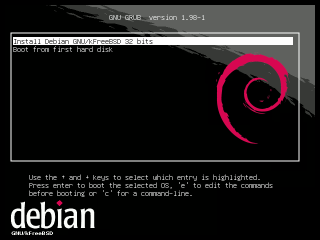
\includegraphics{image201008/kfreebsd-installer.png}
\caption{Debian GNU/kFreeBSD$B$N(BDebian$B%$%s%9%H!<%i(B}\label{debinstaller}
\end{center}
\end{figure}

$B%$%s%9%H!<%kCf$N@_Dj$O0J2<$r;XDj$7$F%$%s%9%H!<%k$7$^$7$?!#(B

\begin{itemize}
 \item locale$B$O!V(BC$B!W!#!J8=;~E@$N%$%s%9%H!<%i$G$O!V(BC$B!W$H!V(BEnglish$B!W$N$_$N(B
locale$B$7$+;XDj$G$-$J$$$?$a!#!K(B
 \item $B%?%$%`%>!<%s$O(BAsia/Japan$B!#(B
 \item $B%$%s%9%H!<%k$O!V(BStandard system utilities$B!W(B(=Base System)$B$N$_!#(B
\end{itemize}

\subsection{$B=i2s5/F0(B}
\subsubsection{$BA0=`Hw(B}
X Window System$B$r%$%s%9%H!<%k$7$F$$$J$$$?$a!":F5/F08e$O%3%s%=!<%k4D6-$G(B
$B5/F0$7$^$9!#(B
$B5/F0;~$K(BDHCP$B%/%i%$%"%s%H$,5/F0$9$k$?$a!"M-@~(BLAN$B4D6-$G$"$l$P(BIP$B%"%I%l%9$r<+F0$G(B
$B<hF@$7$F%M%C%H%o!<%/$K$D$J$,$j$^$9!#(B($B0JA0$O<jF0$G(Bdhclient$B$r5/F0$7$J$$$H(B
$B$D$J$,$i$J$+$C$?!#(B)

$B%+!<%M%k5/F08e$K%$%s%9%H!<%i$G:n@.$7$?%f!<%6$G%m%0%$%s$7!":GDc8BI,MW$J0J2<$N(B
$B%Q%C%1!<%8$r%$%s%9%H!<%k$7@_Dj$7$^$9!#(B

\begin{commandline}
$ su
# apt-get update
# apt-get install sudo vim
# visudo
\end{commandline}

\subsubsection{$B%+!<%M%k$N99?7(B}

$B%+!<%M%k$N5/F0%a%C%;!<%8$rD/$a$F$$$k$H(BCPU$B$,(B1$B$D$7$+G'<1$7$F$$$J$$$h$&$K8+$($^$9!#(B
$B8=:_5/F0Cf$N%+!<%M%k$H(BCPU$B$NG'<1?t$r3NG'$9$k$H$d$O$j(B1$B$D$7$+G'<1$7$F$$$^$;$s!#(B

\begin{commandline}
$ uname -a

GNU/kFreeBSD deb-NorTP60 7.3-1-686 #0
Tue Jul 20 02:12:21 CEST 2010 i686 i386
Genuine Intel(R) CPU           T2400  @ 1.83GHz GNU/kFreeBSD
\end{commandline}

\begin{commandline}
$ cat /proc/cpuinfo

processor   : 0
vendor_id   : GenuineIntel
cpu family  : 6
model       : 7
model name  : Genuine Intel(R) CPU           T2400  @ 1.83GHz
stepping    : 8
flags       : fpu vme de pse tsc msr pae mce cx8 apic sep mtrr pge mca
              cmov pat b19 b21 mmxext mmx fxsr xmm b26 b27 b28 b29 3dnow
cpu MHz     : 1828.76
bogomips    : 1828.76
\end{commandline}

$B8=:_MxMQ$G$-$k%+!<%M%k$r8!:w$9$k$H0J2<$N8uJd$,=P$F$-$^$9!#(B

\begin{commandline}
$ apt-cache search kfreebsd-image-*

kfreebsd-headers-7.3-1-486 - header files for kernel of FreeBSD 7.3
kfreebsd-headers-7.3-1-686-smp - header files for kernel of FreeBSD 7.3
kfreebsd-headers-7.3-1-686 - header files for kernel of FreeBSD 7.3
kfreebsd-image-7-486 - kernel of FreeBSD 7 image
kfreebsd-image-7-686-smp - kernel of FreeBSD 7 image
kfreebsd-image-7-686 - kernel of FreeBSD 7 image
kfreebsd-image-7.3-1-486 - kernel of FreeBSD 7.3 image
kfreebsd-image-7.3-1-686-smp - kernel of FreeBSD 7.3 image
kfreebsd-image-7.3-1-686 - kernel of FreeBSD 7.3 image
kfreebsd-headers-8.0-1-486 - header files for kernel of FreeBSD 8.0
kfreebsd-headers-8.0-1-686-smp - header files for kernel of FreeBSD 8.0
kfreebsd-headers-8.0-1-686 - header files for kernel of FreeBSD 8.0
kfreebsd-image-8-486 - kernel of FreeBSD 8 image
kfreebsd-image-8-686-smp - kernel of FreeBSD 8 image
kfreebsd-image-8-686 - kernel of FreeBSD 8 image
kfreebsd-image-8.0-1-486 - kernel of FreeBSD 8.0 image
kfreebsd-image-8.0-1-686-smp - kernel of FreeBSD 8.0 image
kfreebsd-image-8.0-1-686 - kernel of FreeBSD 8.0 
\end{commandline}

$B%7%s%0%k%W%m%;%C%5MQ$H%^%k%A%W%m%;%C%5MQ$N%+!<%M%k$OJL!9$N$h$&$G$9$N$G(B
$B%^%k%A%W%m%;%C%5MQ%+!<%M%k$r%$%s%9%H!<%k$7!":F5/F0$7$^$9!#(B
\footnote{HyperThreading$B$N%;%-%e%j%F%#>e$N@H<e@-$KBP1~$9$k$?$a(BFreeBSD$BK\2H$,(B
$B%j%j!<%9$9$k%+!<%M%k$O(BHyperThreading$B$,%G%U%)%k%H$G(BOFF$B$K$J$C$F$$$^$9!#(B
Debian GNU/kFreeBSD$B$G%G%U%)%k%H$,(BOFF$B$G$"$k$+$OBP1~(BCPU$B$r;}$C$F$$$J$$$?$a(B
$B3NG'$G$-$F$$$^$;$s!#(B}

$B%+!<%M%k$N%$%s%9%H!<%k=hM}$G(Bgrub2$B$b%"%C%W%G!<%H$5$l$^$9!#(B
\footnote{kfreebsd-image-8.0-1-686-smp$B$r%$%s%9%H!<%k$7$F$_$^$7$?$,!"(B
$B%$%s%9%H!<%k8e$K(B/$B$X%Q!<%F%#%7%g%s$r%^%&%s%H$9$k=hM}$K<:GT$7(B
$B5/F0$G$-$^$;$s$G$7$?!#(BFreeBSD 8.0 Release Note$B$K!V(B''dangerously dedicated'' mode for the UFS file system is no longer supported. Important: Such disks will need to be reformatted to work with this release.$B!W(B
$B$H$$$&5-=R$,$"$k$?$a!"(B7.3$B$+$i(B8.0$B$X$N%+!<%M%k%"%C%W%0%l!<%I$O(B
$B>/$7Fq$7$$$h$&$G$9!#(B}

\begin{commandline}
$ sudo apt-get install kfreebsd-image-7.3-1-686-smp
$ sudo reboot
\end{commandline}

$B:F5/F0$7!"%+!<%M%k$H(BCPU$B$NG'<1?t$r3NG'$7$^$9!#(B

\begin{commandline}
$ uname -a

GNU/kFreeBSD deb-NorTP60 7.3-1-686-smp #0
Tue Jul 20 02:43:20 CEST 2010 i686 i386
Genuine Intel(R) CPU           T2400  @ 1.83GHz GNU/kFreeBSD
\end{commandline}

\begin{commandline}
$ cat /proc/cpuinfo

processor   : 0
vendor_id   : GenuineIntel
cpu family  : 6
model       : 7
model name  : Genuine Intel(R) CPU           T2400  @ 1.83GHz
stepping    : 8
processor   : 1
vendor_id   : GenuineIntel
cpu family  : 6
model       : 7
model name  : Genuine Intel(R) CPU           T2400  @ 1.83GHz
stepping    : 8
flags       : fpu vme de pse tsc msr pae mce cx8 apic sep mtrr pge mca
              cmov pat b19 b21 mmxext mmx fxsr xmm b26 b27 b28 b29 3dnow
cpu MHz     : 1828.76
bogomips    : 1828.76
\end{commandline}

\subsection{Xorg$B$N%$%s%9%H!<%k(B}
X Window System$B4D6-$,F|>o$r2a$4$9$?$a!"(Bxorg$B$r%$%s%9%H!<%k$7$^$9!#(B
$B$7$+$7%Q%C%1!<%8$N%$%s%9%H!<%k=hM}$G0J2<$N%(%i!<$,H/@8$7!"ESCf$G%$%s%9%H!<%k$,(B
$BDd;_$7$^$7$?!#(B

\begin{commandline}
$ sudo apt-get install xorg
Setting up hal (0.5.14-3) ...
Reloading system message bus config...
Failed to open connection to "system" message bus:
Failed to connect to socket /var/run/dbus/system_bus_socket: Connection refused
invoke-rc.d: initscript dbus, action "force-reload" failed.
Starting Hardware abstraction layer: haldinvoke-rc.d: initscript hal,
action "start" failed.
dpkg: error processing hal (--configure):
 subprocess installed post-installation script returned error exit status 1
\end{commandline}

\subsubsection{$BBP1~(B}

$B>e5-$O(Bhal$B$N%$%s%9%H!<%k$N8e=hM}$G(Bdbus$B$N@_Dj$r:FFI$_9~$_$7$h$&$H$7$F%(%i!<$,(B
$BH/@8$7$?$?$a!"%Q%C%1!<%8$N%$%s%9%H!<%k$,Dd;_$7$^$7$?!#(B
\footnote{\url{http://bugs.debian.org/cgi-bin/bugreport.cgi?bug=469528}}

ps$B%3%^%s%I$G(Bdbus$B%W%m%;%9$,$$$k$+3NG'$9$k$HB8:_$7$^$;$s!#(B
$B%P%0=$@5$O$^$@9T$o$l$F$$$J$$$?$a!"$H$j$"$($:$NA<CV$H$7$F(B
$B!V(B{\$} sudo /etc/init.d/dbus start$B!W$r<B9T$7$F(Bdbus$B$r5/F0$7(B
$B:FEY!V(B{\$} sudo apt-get install xorg$B!W$r;n$_$k$H<!$O0J2<$N%(%i!<$K(B
$BJQ$o$j$^$7$?!#(B

\begin{commandline}
$ sudo /etc/init.d/dbus start
$ sudo apt-get install xorg
Setting up xserver-xorg (1:7.5+6) ...
invoke-rc.d: initscript hal, action "restart" failed.
dpkg: error processing xserver-xorg (--configure):
subprocess installed post-installation script returned error exit status 1
\end{commandline}

$B:#EY$O(Bxserver-xorg$B$N%$%s%9%H!<%k$N8e=hM}$G(Bhal$B$HF1MM$N%(%i!<$,H/@8$7$?$?$a!"(B
$B:FEY(Bhal$B$HF1MM$K0J2<%3%^%s%I$r<B9T$7!"(Bxorg$B$N%$%s%9%H!<%k$O40N;$7$^$7$?!#(B

\begin{commandline}
$ sudo /etc/init.d/dbus start
$ sudo apt-get install xorg
\end{commandline}

\subsubsection{X Window System$B5/F05Z$S@_Dj(B}

$B$3$N>uBV$G(Bstartx$B%3%^%s%I$r<B9T$9$k$H(BX Window System$B$N5/F0$K@.8y$7$^$7$?!#(B
$B$7$+$7!V(B/etc/X11/xorg.conf$B!W$N@_Dj$r3NG'$7$h$&$H$9$k$H%U%!%$%k<+BN$,(B
$BB8:_$7$J$$$?$a(Bxorg.conf$B$r<jF0$G:n@.$7$^$9!#(B

\begin{commandline}
$ sudo X -config
$ sudo cp xorg.conf.new /etc/X11/xorg.conf
\end{commandline}

$B:FEY(Bstartx$B$r<B9T$7!":n@.$7$?(Bxorg.conf$B$rMQ$$$F(BX Window System$B$N5/F0$,(B
$B3NG'$G$-$^$7$?!#!V(B/var/log/Xorg.0.log$B!W$r3NG'$7(B'(EE)'$B$NItJ,$O$J$$$?$a!"(B
$BF0:n$O@5>o$G$9!#(B

\subsubsection{gdm$B$N%$%s%9%H!<%k(B($BCGG0(B)}

$B%m%0%$%s2hLL$b(BGUI$B$G9T$$$?$$$N$G(Bgdm$B$r%$%s%9%H!<%k$7$^$9!#(B

\begin{commandline}
$ sudo apt-get install gdm
\end{commandline}

gdm$B$r%$%s%9%H!<%k$7(Breboot$B$;$:$K(Bgdm$B%3%^%s%I$r<B9T$9$k$H%^%&%9!"%-!<%\!<%I$O(B
$BLdBj$J$/F0:n$7$^$9!#(B

reboot$B8e!"<+F0$G(Bgdm$B$,5/F0$9$k$N$G$9$,(Bgdm$B$N%m%0%$%s2hLL$G%^%&%9$OF0$-$^$9$,(B
$B%-!<%\!<%I$,F0:n$7$^$;$s!#(B(USB$B%-!<%\!<%I$bF0:n$7$J$+$C$?!#(B)

$BITK\0U$J$,$i(Bgdm$B$K$h$k%m%0%$%s$OD|$a(Bstartx$B$K$h$k(B X Window System$B$N5/F0$K(B
$B@Z$jBX$($k$3$H$K$7$^$7$?!#$7$+$7$3$N>uBV$G$O%+!<%M%k$N5/F0D>8e$K(Bgdm$B$,(B
$B>!<j$K5/F0$7%-!<%\!<%IF~NO$,$G$-$J$/$J$k$?$a2>A[%3%s%=!<%k$K@Z$jBX$($k$3$H$b(B
$B$G$-$9!"(Bgdm$B$r(Bpurge$B$G$-$^$;$s!#(B

$B$=$N$?$a!"0lEYEE8;%9%$%C%A$rD92!$7$7$F(BPC$B$rDd;_!":F5/F0$7$F(Bgdm$B$,5/F0$9$kA0$K(B
$B!V(BCtrl + Alt + F1$B!W$rO"BG$7$F$J$s$H$+2>A[%3%s%=!<%k$KF~$j0J2<$r<B9T$7$F(Bgdm$B$r(B
purge$B$7$^$7$?!#(B

\begin{commandline}
$ sudo apt-get purge gdm
\end{commandline}

\subsection{$B%G%9%/%H%C%W4D6-$N9=C[(B}

$BE}9g%G%9%/%H%C%W4D6-$G$"$k!V(BXfce4$B!W$r%$%s%9%H!<%k$7!"(Bstartx$B$G(BXfce4$B$r(B
$B5/F0$9$k$h$&$K(B.xinitrc$B$r5-=R$7$^$9!#(B
.xinitrc$B$O<B9T8"$,I,MW$J$?$a!"<B9T8"$rIUM?$7$^$9!#(B

\begin{commandline}
$ sudo apt-get xfce4 xfce4-goodies
$ vim ~/.xinitrc
exec xfce4-session

$ chmod 744 ~/.xinitrc
$ startx
\end{commandline}

\subsection{$BF|K\8l4D6-(B}

\subsubsection{$BF|K\8l$NI=<((B}

$BF|K\8l%U%)%s%H$r%$%s%9%H!<%k$7$^$9!#(B

\begin{commandline}
$ sudo apt-get otf-ipafont otf-ipaexfont
\end{commandline}

$BF|K\8l4D6-$N!V(Bja\_JP.UTF-8$B!W%m%1!<%k$O%$%s%9%H!<%k$5$l$F$$$J$+$C$?$?$a(B
$BDI2C%$%s%9%H!<%k$7$^$9!#(B

\begin{commandline}
$ sudo apt-get locales-all
\end{commandline}

startx$B%3%^%s%I$G(BX Window System$B$r5/F0$9$k$?$a(Blocale$B$N@_Dj$r(B.xinitrc$B$KDI5-$7$^$9!#(B
Xfce4$B$r=*N;$7$F:FEY(Bstartx$B%3%^%s%I$r<B9T$9$k$H(BXfce4$B$,F|K\8l4D6-$G5/F0$7$^$9!#(B

\begin{commandline}
$ vim ~/.xinitrc    

export LANGUAGE='ja_JP.UTF-8'
export LC_ALL='ja_JP.UTF-8'
export LANG='ja_JP.UTF-8'
exec xfce4-session

$ startx
\end{commandline}

\subsubsection{$BF|K\8lF~NO(B}

$BF|K\8lF~NO4D6-$H$7$F(Buim$B$r;HMQ$7$?$$$?$a!"(Buim$B$N%$%s%9%H!<%k$H@_Dj$r$7$^$9!#(B

\begin{commandline}
$ sudo apt-get install uim uim-anthy
$ vim ~/.xinitrc

export LANGUAGE='ja_JP.UTF-8'
export LC_ALL='ja_JP.UTF-8'
export LANG='ja_JP.UTF-8'

export XMODIFIRES='@im=uim'
export GTK_IM_MODULE='uim'
export QT_IM_MODULE='uim'

exec xfce4-session

$ startx
\end{commandline}

\subsection{$B3+H/4D6-$N%$%s%9%H!<%k(B}

Debian GNU/kFreeBSD$B$N%G%P%C%0$KI,MW$J%3%s%Q%$%i!"%Q%C%1!<%8$N:n@.%D!<%k$r(B
$B%$%s%9%H!<%k$7$^$9!#(B

\begin{commandline}
$ sudo apt-get update
$ sudo apt-get install gcc g++ gdb make
$ sudo apt-get install build-essential pbuilder debian-keyring
\end{commandline}

deb$B%Q%C%1!<%8$N%S%k%I$,$G$-$k$+(Btcsh$B$r%S%k%I$7$F3NG'$7$^$9!#(B

\begin{commandline}
$ apt-get source tcsh
$ sudo apt-get build-dep tcsh
$ cd tcsh-6.17.00
$ dch
$ debuild -i -us -uc -b
$ sudo dpkg -i tcsh_6.17.00-3.1_kfreebsd-i386.deb
\end{commandline}

\subsection{Debian$BJY6/2q;qNA$N%S%k%I4D6-(B}

Debian$BJY6/2q$G$N869F$O(Btex$B$r:NMQ$7$F$$$k$?$a!"869F%U%!%$%k$N%S%k%I4D6-$r(B
$B9=C[$7$^$9!#(B

tex$B$N%S%k%I$K$O(Bconrtib$B!"(Bnon-free$B$N%Q%C%1!<%8$,I,MW$J$?$a!"(B
apt-line$B$r=$@5$7$^$9!#(B

\begin{commandline}
$ sudo vim /etc/apt/sources.list
# deb http://ftp.jp.debian.org/debian/ squeeze main

deb http://ftp.jp.debian.org/debian/ squeeze main contrib non-free
deb-src http://ftp.jp.debian.org/debian/ squeeze main contrib non-free

deb http://security.debian.org/ squeeze/updates main
deb-src http://security.debian.org/ squeeze/updates main
\end{commandline}

$BI,MW$J%Q%C%1!<%8$r%$%s%9%H!<%k$7$^$9!#(B

\begin{commandline}
$ sudo apt-get install git-core
$ sudo apt-get install gs gs-esp gs-cjk-resource
$ sudo apt-get install ptex-bin xdvik-ja dvipsk-ja
$ sudo apt-get install okumura-clsfiles vfdata-morisawa5
$ sudo apt-get install texlive-latex-extra
$ sudo apt-get install poppler-data
$ sudo apt-get install evince
\end{commandline}

$B;qNA$r%@%&%s%m!<%I$7!"%S%k%I$7$^$9!#(B

\begin{commandline}
$ cd
$ git clone git://git.debian.org/git/tokyodebian/monthly-report.git/
$ cd monthly-report
$ make
\end{commandline}

\subsection{$B$=$NB>$NF|>o4D6-$N9=C[(B}

$B$=$NB>$N$h$/;H$&%=%U%H$r%$%s%9%H!<%k$7$^$9!#(B

\begin{commandline}
$ sudo apt-get install emacs emacs23-el
$ sudo apt-get install sylpheed sylpheed-i18n
$ sudo apt-get install iceweasel iceweasel-l10n-ja
$ sudo apt-get install audacious audacity
$ sudo apt-get install gxine
$ sudo apt-get install jd
$ sudo apt-get install gftp
\end{commandline}

\subsection{$B%G%P%$%9%I%i%$%P(B}
audacious$B$O2;3Z:F@8%=%U%H$J$N$G$9$,!"<B9T$7$F$b2;$,LD$j$^$;$s!#(B
$B%5%&%s%I%I%i%$%P$r%m!<%I$7$F$$$k$+3NG'$9$k$?$a!V(Bkldstat$B!W$r<B9T$7$^$9!#(B
\footnote{FreeBSD$B%+!<%M%k$GFI$_9~$_Cf$N%+!<%M%k%b%8%e!<%k$N0lMw$r=PNO$9$k(B
$B%3%^%s%I$O(Bkldstat$B$G$9$,!"(BDebian GNU/KFreeBSD$B$G$O(Blsmod$B$,(Bkldstat$B$N%j%s%/$K(B
$B$J$C$F$$$k$?$a(Blsmod$B$G$b0lMw$r=PNO$G$-$^$9!#(B}

\begin{commandline}
$ kldstat
 1   10 0xc0400000 890000   kfreebsd-7.3-1-686-smp.gz
 2    1 0xc0d9c000 57fdc    acpi.ko
 3    1 0xc5c7a000 67000    radeon.ko
 4    1 0xc5ce1000 14000    drm.ko
\end{commandline}

$B%5%&%s%I%I%i%$%P$,%m!<%I$5$l$F$$$J$$$?$a%m!<%I$7$^$9!#(B
\footnote{snd\_hda$B$O(BIntel945$B%A%C%W%;%C%H$G2;$rLD$i$9$?$a$KI,MW$J(B
$B%5%&%s%I%I%i%$%P$G$9!#0[$J$k%5%&%s%I%A%C%W$rMxMQ$7$F$$$k>l9g$O(B
$B4D6-$K9g$o$;$F%m!<%I$7$F$/$@$5$$!#(B}

\begin{commandline}
$ sudo kldload snd_hda
$ kldstat
 1   10 0xc0400000 890000   kfreebsd-7.3-1-686-smp.gz
 2    1 0xc0d9c000 57fdc    acpi.ko
 3    1 0xc5c7a000 67000    radeon.ko
 4    1 0xc5ce1000 14000    drm.ko
 5    1 0xc611f000 1a000    snd_hda.ko
 6    1 0xc6139000 40000    sound.ko
\end{commandline}

$B2;$,LD$k$3$H$O3NG'$G$-$^$7$?$,!":F5/F0$9$k$H%5%&%s%I%I%i%$%P$,FI$_9~$^$l$F(B
$B$$$J$$>uBV$K$J$j$^$9!#$=$N$?$a!V(B/etc/modules$B!W%U%!%$%k$K%+!<%M%k5/F0;~$K(B
$B<+F0$GFI$_9~$`%I%i%$%P$r@_Dj$7$^$9!#(B
\footnote{Debian GNU/kFreeBSD$B$K(B/sbin/modprobe$B%3%^%s%I$O$"$k$N$G$9$,(B
/sbin/kldload$B$N%j%s%/$K$J$C$F$$$k$?$a!"(Bmodprobe$B$r$7$?$@$1$G:F5/F08e$b(B
$B<+F0$G%b%8%e!<%k$rFI$_9~$`$h$&$K$O$J$C$F$$$J$$$h$&$G$9!#(B}

\begin{commandline}
$ sudo vim /etc/modules
# /etc/modules: kernel modules to load at boot time.
#
# This file should contain the names of kernel modules that are
# to be loaded at boot time, one per line.  Comments begin with
# a ``#'', and everything on the line after them is ignored.
snd_hda.ko
\end{commandline}

\subsection{$B:#8e$N2]Bj(B}
Debian GNU/kFreeBSD$B$G%;%C%H%"%C%W:n6H$r9T$$$^$7$?$,F|>o@83h$rAw$k$K8~$1$F(B
$B$$$/$D$+2]Bj$,;D$C$F$$$^$9!#(B

\begin{itemize}
 \item Web$B%V%i%&%6$G$N(BFlash$B$N:F@8(B(Adobe$B8x<0$N(BFlash$B%P%$%J%j$K(BFreeBSD$BHG$O(B
$B$^$@$J$$(B)
 \item $B%S%G%*:F@8(B($B1GA|$,Mp$l$k!#$*$=$i$/(Bcodec$B$NLdBj(B)
\end{itemize}

$B:#8e$K$`$1$?<h$jAH$_$H$7$F0J2<$r;n$7$F$$$-$?$$$G$9!#(B

\begin{itemize}
 \item Linux$B%P%$%J%j8_495!G=(B
 \item $B2>A[2=5!G=(B(Jail$B!"(BVirtualBox$B!"(Bqemu)
 \item ZFS
\end{itemize}

\subsection{$B4D6-9=C[$r=*$($F(B}
$B%$%s%9%H!<%i$N@0Hw$b?J$s$G$*$j!"(BX Window System$B$NF3F~8e$O(BDebian GNU/Linux$B$H(B
$B$J$s$iJQ$o$i$J$$<j=g$G4D6-9=C[$,$G$-$^$7$?!#(B

$B$?$@LdBj$,H/@8$7$?$H$-$K(BFreeBSD$B%+!<%M%k$H(BDebian$B$NN>J}$NCN<1$,I,MW$J$?$a!"(B
$B860x$rD4$Y$k$N$,BgJQ$G(BFreeBSD$B$H(BDebian$B$NN>J}$N>pJs8;$KEv$?$C$F$J$s$H$+(B
$B2r7h$7$^$7$?!#(B

$B%P%0Js9p$,$"$k$HF1$8$H$3$m$G$D$^$:$$$F$$$k?M$H>pJs$r6&M-$G$-$k$N$G(B
$B$G$-$k$@$1%P%0Js9p$O>e$2$^$7$g$&!#(B

Debian GNU/kFreeBSD$B$OIJ<A$b=y!9$K>e$,$C$F$-$F$*$j!"(BSqueeze$B$G5;=Q%W%l%S%e!<(B
$B07$$$N%j%j!<%9$,$5$l$kM=Dj$G$9!#(B\footnote{\url{http://www.debian.org/News/2010/20100806}}
$B$_$J$5$s$b$<$R(BDebian GNU/kFreeBSD$B$r%G%P%C%0$7$F(BSqueeze$B%j%j!<%9$^$G$KIJ<A$r(B
$B9b$a$^$7$g$&!#(B

\subsection{$B;29M;qNA(B}
\begin{itemize}
 \item $BEl5~%(%j%"(B Debian $B=PD%JY6/2q(B $BH/I=%9%i%$%I(B($B4d>>?.MN(B) : \url{http://tokyodebian.alioth.debian.org/pdf/debianmeetingresume201006-iwamatsu-presentation.pdf}
 \item Debian wiki : \url{http://wiki.debian.org/Debian\_GNU/kFreeBSD\_FAQ}
\end{itemize}

\dancersection{Emdebian $B$K$D$$$F(B -$B4X@>(B Debian $BJY6/2q;22C<TCf4VJs9p(B- }{$B$?$J$+$H$7$R$5(B}

\subsection{$BA0=q$-(B}

$B$3$N;qNA$O!"I.<T$,(B Emdebian $B$r;H$&>e$GJY6/$7$?;v$r5-:\$7$F$$$^$9!#$^$@$^(B
$B$@!"40A4$KM}2r$7$?$o$1$G$O$J$/!"ItJ,ItJ,$G$7$+(BEmdebian$B$r;H$($F$$$^$;$s$,!"(B
$BCf4VJs9p$H8@$&;v$G$4MF<O$/$@$5$$!#(B

\subsection{Emdebian $B$C$F(B?}

Emdebian (Embedded Debian)$B$O!"(BDebian GNU/Linux$B$r85$K!"AH9~$_5!4oMQES$K:G(B
$BE,2=$7$F$$$/%W%m%8%'%/%H$G$9!#(B

Debian GNU/Linux $B$O!"$^$:(B Debian$B<+?H$,%^%k%A%"!<%-%F%/%A%c(B($BJY6/2q2]Bj(B1)$B$K(B
$BBP1~$7$F$$$^$9!#$^$?!"$I$N%Y%s%@!<$+$i$bFHN)$7$F$*$j!"(BDebian $B<R2q7@Ls!"$*(B
$B$h$SKDBg$JMxMQ2DG=%=%U%H%&%'%"$OMM!9$JA*Br;h$r2DG=$K$7$^$9$,!"%G%9%/%H%C(B
$B%W4D6-(B($BBg$-$J%O!<%I%G%#%9%/$H%a%b%j(B)$B$K8~$1$i$l$F$$$^$9!#(B

`Embedded Debian`$B$O!"(BDebian $B$N%a%j%C%H$r3h$+$7$D$D!"AH9~$_5!4o$NMM$J>.$5(B
$B$$%7%9%F%`8~$1$K(B Debian $B$r7ZNL$K$9$k$b$N$G$9!#(B

($B>e5-$O!"(B\url{http://www.emdebian.org/}$B$+$i0ULu$7$?$b$N$G$9(B)

\subsubsection{$BJY6/2q2]Bj(B1: Debian $B$,F0:n$9$k(B CPU$B!"%?!<%2%C%H5!4o(B}

\url{http://www.jp.debian.org/ports/}$B$+$i!"(BDebian $B$N0\?"HG$K4X$9$k>pJs$,(B
$BF@$i$l$^$9!#(B

\begin{itemize}
 
 \item Intel x86 / IA-32 (i386) - 1$BHV?H6a$G;H$o$l$F$$$^$9$M!#(B 
 \item (Motorola 68k (m68k)) - Etch $B0J9_$N%j%j!<%9$K$O4^$^$l$F$$$^$;$s!#(B
 \item  Sun SPARC (sparc)

 \item  Alpha (alpha)
 \item  Motorola/IBM PowerPC (powerpc)
 \item  ARM (arm $B$*$h$S(B armel) - $B:#2s<h$j>e$2$k(B CPU $B$G$9!#(B
 \item  MIPS CPUs (mips$B$H(Bmipsel)
 \item  HP PA-RISC (hppa)
 \item  IA-64 (ia64)
 \item  S/390 (s390)
 \item  AMD64 (amd64)
\end{itemize}

Debian$B$O!"%+!<%M%k$K(BLinux$B%+!<%M%k$r;H$$$^$9$,!"(BDebian GNU/kFreeBSD$B$NMM$K!"(B
$B%+!<%M%k$K(BFreeBSD$B$N%+!<%M%k$r;H$&$b$N$b$"$j$^$9!#(B

\subsubsection{$BJY6/2q2]Bj(B2: $B3'$5$s!">e5-$NFb!";H$C$?;v$N$"$k%"!<%-%F%/%A%c$r65$($F$/$@$5$$!#(B}

$B$J$*!"(BEmdebian $B$O!"2<5-$N%"!<%-%F%/%A%c$,MxMQ2DG=$G$9!#(B

i386$B!"(Bamd64$B!"(Bpowerpc$B!"(Barmel$B!"(Bmips$B!"(Bmipsel

\subsection{Emdebian $B$O2?$r:n$C$F$$$k$+(B($B2?$r:n$m$&$H$7$F$$$k$+(B)$B!#(B}

\begin{description}
 \item[Toolchains]
 
           gcc$B$r=i$a$H$7$?!"%S%k%I:Q$_$N3+H/4D6-$G$9!#(B
\end{description}

\begin{description}
 \item[Smaller packages] 
  \begin{description}
   \item[Emdebian Grip - binary-compatible with Debian]

              ($B:#2s$*OC$7$9$k$b$N$O$3$l$G$9(B)

              $B$3$l$O!"(BDebian $B$+$i%$%s%9%H!<%k$G$-$k(B($BMW$9$k$K(Bdebootstrap $B$G%$%s%9%H!<%k$G$-$k(B)$B$b$N$G$9!#(B

   \item[Emdebian Crush - cross-built, customised Emdebian installations without perl] 

              Web $B%Z!<%8$K$h$k$H!"(BBusybox $B$r%Y!<%9$K$7$?(B root filesystem
              $B$H$N;v$G$9!#(B

              Busybox $B$G$"$k$?$a!"(BDebian $B$=$N$b$N$H9=@.$,JQ$o$C$F$$$k;v$,(B
              $B9M$($i$l$^$9$,!"(BEmdebian Grip $B$HHf$Y$k$H!"$b$C$HMFNL$O>.$5(B
              $B$$$H9M$($F$$$^$9!#(B
  \end{description}
\end{description}

\begin{description}
 \item[Cross building tools] 

            $B$=$NL>$NDL$j!"%/%m%93+H/%D!<%k$G$9!#(B

            $B!V%/%m%93+H/!W$H$O!"Nc$($P%Q%=%3%s(B(i386)$B>e$G!"(BARM $B$N%P%$%J%j(B
            $B$r@8@.$9$kMM$J!"%[%9%H(B($B%3%s%Q%$%k(B)$B4D6-$H%?!<%2%C%H(B($B<B9T(B)$B4D6-(B
            $B$N(BCPU$B$d(BOS$B$,0[$J$k>l9g$N3+H/$r8@$$$^$9!#(B

            $BAH9~$_5!4o$O!"$=$NKX$I$,%/%m%93+H/$G:n$j$^$9!#(B

            $BB>J}!"%[%9%H4D6-$H%?!<%2%C%H4D6-$,F1$8!"C1=c$K8@$($P!"(Bi386$B>e(B
            $B$G!"(Bi386$B>e$GF0$/%=%U%H%&%'%"$r3+H/$9$k>l9g$O!"!V%;%k%U3+H/!W(B
            $B$H8@$$$^$9!#(B

            Emdebian$B$O!"(BDebian$B@55,$N$b$N$HF14|$7$J$,$i!"%/%m%93+H/4D6-$K(B
            $B>GE@$rEv$F$F$$$^$9!#(Bi386$B$H(B amd64$B%"!<%-%F%/%A%c>e$G!"(Barm,
            ia64, m68k, mips, mipsel, powerpc, sparc$B$N%S%k%I$,2DG=$G$9!#(B
\end{description}

\begin{description}
 \item[Root filesystem generation is based on multistrap package.]

            multistrap$B$O!"(BEmdebian$B$G(Broot filesystem$B$r:n$k$&$($G$N%a%$%s$H(B
            $B$J$k%D!<%k$G$9!#(B

            ($B$4$a$s$J$5$$!"(Bmultistrap $B$O$^$@I.<T$,==J,$KJY6/$G$-$F$$$^$;(B
            $B$s!D(B)
\end{description}

Emdebian$B<+?H!"$^$@:n6HCf$N$b$N$,B?$/!"6(NO<T$rJg=8$7$F$$$^$9!#(B

\url{http://www.emdebian.org/emdebian/helpout.php} $B$3$N%Z!<%8$K!"(B
Emdebian$B$N(BToDo($B%P%0%j%9%H(B)$B$,$"$j$^$9!#(B

\subsection{$B$J$<!"!VAH9~$_(B Linux$B!W$J$N$+(B?($B$J$<!VAH9~$_(B Debian$B!W$J$N$+(B?)}

$BM}M3$O?M$=$l$>$l$G$9$,!"I.<T<+?H$,6/$/46$8$k$N$O!"AH9~$_(BLinux$B$O!"%W%m%0%i(B
$B%`$NF0:n3NG'$,MF0W$K$J$j!"%=%U%H%&%'%"$NIJ<A$r3NJ]$7$d$9$/$J$k$H8@$&;v$G(B
$B$9!#(B

$BNc$($P!"F|K\$NAH9~$_5!4o$G;H$&(BOS$B$K$O(BiTron$B$r;H$&;v$,B?$$$G$9!#3$30$@$H(B
VxWorks$B$r;H$&;v$,B?$$$G$9!#(BiTron$B$r;H$C$?3+H/$N>l9g!"(BiTron$B$N%7%9%F%`%3!<(B
$B%k$O!"(BPC$B$G$O%7%_%e%l!<%?(B($B$"$k$$$O%(%_%e%l!<%?(B)$B$r;H$o$J$$8B$j!"F0$-$r4^$a(B
$B$?F0:n3NG'$O=PMh$^$;$s!#(B

$B$=$N$?$a!"(BJTAG$BEy$N%G%P%C%,$r;H$C$F!"<B5!$K%W%m%0%i%`$r>F$-$3$s$G%G%P%C%0(B
$B$9$k;v$,KX$I$G$9!#(B

$BAH9~$_(BLinux$B$N>l9g!"(Bi386 $BHG(B Linux $B$G!"$"$kDxEYF0$-$b4^$a$?%G%P%C%0$b2DG=$K(B
$B$J$j$^$9!#(B

ARM$BHG(BLinux$B8~$1$N%W%m%0%i%`$r:n$k$H$7$F!"0l!9(BARM$BHG%W%m%0%i%`$r%S%k%I$7$F(B
ARM CPU$B$J%?!<%2%C%H%\!<%I$KE>Aw$9$k$h$j$b!"(Bi386$BHG(BLinux$B$GAFJ}%G%P%C%0$7$F(B
$B$*$-!"%?!<%2%C%H4D6-$G$O<B:]$N%?!<%2%C%H$J$i$G$O$N%G%P%C%0$KCmNO$9$l$P!"(B
$B%G%P%C%0;~4V$r:o8:$G$-$^$9!#%G%P%C%0;~4V$r:o8:$G$-$k$H8@$&;v$O!"%=%U%H%&%'(B
$B%"%F%9%HEy$N;~4V$rA}$d$9;v$,=PMh$k$H8@$&;v$G$"$j!"%=%U%H%&%'%"$NIJ<A8~>e(B
$B$K7R$2$k$3$H$,=PMh$^$9!#(B

$B3N$+$K!"%?!<%2%C%H5!4o>e$GA4$FF0:n3NG'$r$9$Y$-$G$9$,!"%?!<%2%C%H5!4o>e$G(B
$B%H%l!<%9%G%P%C%0$r$9$k$h$j$b!"%[%9%H4D6->e$G4pK\E*$J%G%P%C%0$,$G$-$k$N$O(B
$BL%NO$G8z2LE*$G$9!#(B

Linux$B$O!"L5NA$G;HMQ$G$-$^$9$,!"I.<T$O!"M-NA(B/$BL5NA$H$OJL$K!"%=%U%H%&%'%"$N(B
$BIJ<A$r3NJ]$7$d$9$$$H$$$&E@$G!"AH9~$_(BLinux$B$OB>$N(BOS$B$h$j$bM%0L@-$,$"$k$H9M$((B
$B$F$$$^$9!#(B

$B$5$i$K!"AH9~$_(B Debian$B$O!"(BPC$BEy$GF@$?(BDebian$B$NCN<1$r!"AH9~$_5!4o$K$b3h$+$9;v(B
$B$,=PMh$^$9!#%=%U%H%&%'%"$NIT6q9g$N$$$/$D$+$O!"IT47$l$J(B($BL$CN$J(B)$B4D6-2<$G$"$C(B
$B$?;v$K5/0x$9$kIT6q9g$,$"$j$^$9!#IaCJ$+$i;H$$47$l$F$$$k(BOS(Debian)$B$,;H$($k(B
$B;v$b!"%=%U%H%&%'%"$NIJ<A$r3NJ]$9$k>e$G=EMW$J$N$G$9!#(B

$B:G8e$K!"(BDebian$B$O%Y%s%@!<FHN)!"JL$N8@$$J}$r$9$k$H!DE];:$9$k;v$,$J$$$G$9(B :-)$B!#(B

$B!V(BLinux$B4k6H!W$O!"<+<gFHN)$GJb$-B3$1$F$$$k%Y%s%@!<$b$"$l$P!"5[<}9gJ;!"$"$k(B
$B$$$OItLgGd5Q$J$I$G4GHD$,JQ$o$j!"7@Ls$,JQ$o$k>l9g$,$"$j$^$9!#(B

$B!V(BLinux$B4k6H!W$H7@Ls$9$kB&$K$7$F$_$l$P!"(BLinux$B4k6H$H7@Ls$7$?$b$N$N!"$"$kF|(B
$BItLgGd5QEy$G7@Ls@h$,JQ$o$j!":FEY?75,7@Ls$+$i$d$jD>$7!D$H$J$k$N$O<j4V$G$9!#(B
$B$b$7$=$3$GHqMQLL$+$iOC$r$7$J$1$l$P$J$i$J$$$H$9$k$H!"(BLinux$B$r;H$&$3$H<+?H$K(B
$B>C6KE*$K$J$j$^$9!#(B

Debian $B$O!"$=$NMM$J;v$O$"$j$^$;$s$N$G!"0B?4$7$F;H$$B3$1$k$3$H$,=PMh$^$9!#(B

\subsection{Emdebian Grip $B$r;n$7$F$_$k!#(B}

Emdebian Grip $B$r!"(BMINI2440 $B$K%$%s%9%H!<%k$7$F$_$^$7$?!#(B

$B87L)$K8@$&$H!D(B rootfs$B$O(BEmdebian Grip$B$G$9$,!"(BLinux$B%+!<%M%k$O(BEmdebian$B$=$N$b(B
$B$N$G$O$"$j$^$;$s!#$9$_$^$;$s!#$3$l$b0z$-B3$-$NJY6/2]Bj$H$5$;$F$/$@$5$$!#(B

$B<L??$O!"(BMINI2440$B$K(BEmdebian Grip$B$r%$%s%9%H!<%k$7$F!"(Biceweasel$B$G(B
OpenStreetMap$B$N%Z!<%8$r;2>H$7$?$b$N$G$9!#(BARM$B>e$G(BWeb$B%V%i%&%6$,IaDL$K;H$($^(B
$B$9(B($BC"$7CY$$$G$9(B)$B!#(Brootfs$B$O(BSD$B%+!<%I$r;H$C$F$$$^$9!#(B



MINI2440$B$N>\$7$$>pJs$O!"(B\url{http://www.friendlyarm.net/products/mini2440}$B$r;2>H$7$F$/$@$5$$!#(B

\subsubsection{$BI,MW$J$b$N(B}

$B$^$:!"(BMINI2440$B$N(BNAND$B%U%i%C%7%e(BROM$B$N%P%C%/%"%C%W$r<h$k$K$O!";DG0$J$,$i(B
MS-Windows$B>e$GF0$/%=%U%H%&%'%"(B(DNW)$B$,I,MW$G$9!#I.<T$O!"(BNAND$B%U%i%C%7%e(BROM
$B$N%P%C%/%"%C%W$H!"%V!<%H%m!<%@(B(U-Boot)$B=q$-9~$_$K(B($BITK\0U$G$9$,(B)MS-Windows
$B$r;H$$$^$7$?!#(B($B8e$9$_$^$;$s!"(BTeraTerm$B$b;H$$$^$7$?(B)

$BB>$KI,MW$J$b$N$r0J2<$K5-$7$^$9!#(B
\begin{itemize}
 \item MINI2440$BK\BN(B
 \item i386(amd64)$B$J(B Debian
 \item $B%M%C%H%o!<%/(B
 \item $B%7%j%"%k%1!<%V%k(B($B%/%m%9%1!<%V%k(B)
 \item SD$B%+!<%I(B(1GByte~2GByte)(Debian PC$B$+$i%"%/%;%9$9$k$N$G!"%+!<%I%"%@%W%?$bI,MW(B)
\end{itemize}

\subsubsection{MINI2440$B$N(BEmdebian$B2=(B}

\subsubsubsection{MINI2440 NAND $B%U%i%C%7%e$N%P%C%/%"%C%W(B($BI,MW$J$i(B)}

MINI2440$B$O!"9XF~$7$?>uBV$G$O(BNAND$B%U%i%C%7%e(BROM $B$K(BQt/Embedded$B$,%$%s%9%H!<%k(B
$B$5$l$F$$$^$9$N$G!"$b$7I,MW$J$i$P%P%C%/%"%C%W$7$F$/$@$5$$!#(B

\subsubsubsection{Emdebian Grip rootfs $B$N<hF@(B}

\url{http://code.google.com/p/mini2440/wiki/Emdebian}$B$r;29M$K!"(BEmdebian
Grip$B$N(Brootfs$B$r<hF@$7$^$9!#$3$3$G$O(Bdebootstrap$B$r;H$$$^$9$N$G!"E,59(B
apt-get$BEy$G%$%s%9%H!<%k$7$F$*$$$F$/$@$5$$!#(B

Emdebian Grip rootfs $B$O!">e5-(BURL$B$K5-:\$7$F$$$k<j=g$G?J$a$i$l$^$9!D$,!"$3(B
$B$N(BURL$B$G$O!"(BEmdebian Grip$B8~$1(BLinux$B%+!<%M%k%S%k%I$K4X$9$k;v$,L5$$$N$G!"(B
Emdebian Grip$B8~$1$N(BLinux$B%+!<%M%k$r%S%k%I$9$kI,MW$,$"$j$^$9!#(B

\subsubsubsection{MINI2440(Emdebian Grip)$B8~$1(BLinux$B%+!<%M%k$N%S%k%I(B}

MINI2440(Emdebian Grip)$B8~$1(BLinux$B%+!<%M%k$r%S%k%I$9$k$K$O!":GDc8B2<5-$N$b(B
$B$N$,I,MW$G$9!#(B

\begin{enumerate}
 \item Toolchain(gcc)
 \item (MINI2440$B$KBP1~$7$?(B)Linux $B%+!<%M%k%=!<%9(B
\end{enumerate}

$B$G$-$l$P!"$=$l$3$=(BEmdebian$B$G0l7b$K!D$H;W$C$?$N$G$9$,!"I.<T$O(B
\url{http://code.google.com/p/mini2440/downloads/list}$B$+$iF@$i$l$k(B
mini2440-bootstrap-v2.sh$B$H8@$&%7%'%k%9%/%j%W%H$r2~B$$7$F;H$$$^$7$?!#(B

$B$3$N%7%'%k%9%/%j%W%H(B(mini2440-bootstrap-v2.sh)$B$O!"3+H/4D6-(B(CodeSoucery)$B$d(B
MINI2440$B8~$1(BLinux$B%+!<%M%k$r<+F0E*$K%@%&%s%m!<%I$7$F%S%k%I$7$^$9!#(B

$B$J$*!"(Bmini2440-bootstrap-v2.sh$B$O!"(BDebian$B>e$G$b;H$($^$9$,!"(BU-Boot$B$N%=!<%9(B
$B%3!<%I$O%@%&%s%m!<%I$7$^$9$,%S%k%I$O$7$J$$$N$G!"2<5-$NMM$K=$@5$7$F;H$$$^(B
$B$9!#(B

\begin{commandline}
 tosihisa@lavie:~/Downloads$ diff -ca mini2440-bootstrap-v2.sh mini2440-bootstrap-v2.sh.change
 *** mini2440-bootstrap-v2.sh    2010-08-17 17:19:45.000000000 +0900
 --- mini2440-bootstrap-v2.sh.change     2010-08-17 17:19:13.000000000 +0900
 ***************
 *** 72,78 ****
  # compile bits
  cd ${DEST}/uboot/mini2440
  make mini2440_config
 ! # make clean all

  cd ${DEST}/kernel/mini2440

 --- 72,78 ----
  # compile bits
  cd ${DEST}/uboot/mini2440
  make mini2440_config
 ! make clean all

  cd ${DEST}/kernel/mini2440

 tosihisa@lavie:~/Downloads$
\end{commandline}

\subsubsubsection{U-Boot$B$r(BMINI2440$B$K%$%s%9%H!<%k$9$k!#(B}

MINI2440$B$O!"(BSupervivi$B$H8@$&%V!<%H%m!<%@$,(BNOR$B%U%i%C%7%eB&$K$"$j$^$9$,!"(B
NAND$B%U%i%C%7%eB&$K(BU-Boot$B$r%$%s%9%H!<%k$7$^$9!#(B

U-Boot(the Universal Boot Loader)$B$O!"(BLinux $B%+!<%M%k$@$1$G$J$/!"(BELF$B7A<0$G(B
$B$"$l$P%m!<%I$G$-$k%V!<%H%m!<%@$G$9!#$^$?!"%V!<%H%m!<%@$H$7$F$N5!G=$@$1$G(B
$B$O$J$/!"%a%b%jA`:n$,2DG=$J$N$G!"%G%P%C%0%D!<%k$H$7$F$bMxMQ$G$-$^$9!#(B

U-Boot$B$O!"(B\url{http://www.friendlyarm.net/downloads}$B$+$iF~<j$G$-$k%S%k%I(B
$B:Q$_$N%P%$%J%j(B(u-boot\_20100701.zip)$B$r;H$$$^$7$?!#(B

\subsubsubsection{Emdebian Grip $B$r5/F0!D(B}

rootfs$B$r:n$j!"(BLinux $B%+!<%M%k$r%S%k%I$G$-$?$i!"$=$l$i$r(BSD$B%+!<%I$K%3%T!<$7(B
$B$^$9!#(B
U-Boot$B$r(BMINI2440$B$K>F$-$3$a$?$i!"(BLinux$B$r5/F0$7$^$9!#(B

debootstrap $BD>8e$N(BSD$B%+!<%I$G5/F0$7$?>l9g!"40A4$K$O%$%s%9%H!<%k$,40N;$7$F(B
$B$$$^$;$s$N$G!"(BU-Boot$B$N%V!<%H%Q%i%a!<%?$K(B'init=/bin/sh'$B$rM?$($F!"%7%'%k$r(B
$B5/F0$5$;$k$h$&$K$7$^$9!#(B

$B$=$N8e!"(B(MINI2440$B$G5/F0$7$?(BEmdebian$B$G(B)$B%7%'%k$,5/F0$7$?$i!"%M%C%H%o!<%/$,(B
DHCP$B$G3d$j?6$i$l$?>uBV$G!"2<5-$N%3%^%s%I$r<B9T$9$k;v$G(BEmdebian$B$N%$%s%9%H!<(B
$B%k$,7QB3$5$l$^$9!#(B

\begin{commandline}
 sh-3.2# /debootstrap/debootstrap --second-stage
\end{commandline}

$B$3$l$,=*$o$l$P!"(BEmdebian Grip$B$,3Z$7$a$^$9!#(Bapt-get$B$G%=%U%H$rF~$l$F$_$F$/(B
$B$@$5$$!#(B

\subsection{$B=PMh$F$J$$$3$H$@$i$1(B($B:#8e$NJY6/2]Bj(B)}
\begin{itemize}
 \item Toolchain $B$b(B Emdebian $B$N$b$N$r;H$&!#(B
 \item Linux $B%+!<%M%k$b(B Emdebian $BM3Mh$N$b$N$r;H$C$F$_$?$$!#(B
 \item Emdebian Crush $B$r;n$9!#(B
 \item U-Boot $B$O%=!<%9$+$i%S%k%I$7$F;H$&!#(B
 \item $B$3$N;qNA$r=<<B$5$;$k(B($BG/Kv$K$O!D(B)
\end{itemize}

\dancersection{$B:#8e$NM=Dj(B}{Debian JP}

\subsection{$B<!2s$N4X@>(BDebian$BJY6/2q(B}

$B<!2s!"(B2010$BG/(B9$B7n$N4X@>(BDebian$BJY6/2q$O!"(B9$B7n(B26$BF|(B($BF|(B)$B$K<B;\$9$kM=Dj$G$9!#(B
$B$$$D$b$H0c$&>l=j$G$N3+:E$H$J$kM=Dj$G$9$N$G!";vA0$N%"%J%&%s%9$K$4Cm0U$/$@(B
$B$5$$!#(B

% $B:};R$K$9$k$?$a$K!"(B4$B$NG\?t$K$9$kI,MW$,$"$k!#(B
% $B$=$N$?$a$ND4@0(B
\dancersection{$B%a%b(B}{}
\mbox{}\newpage

\printindex
 \cleartooddpage

 \begin{minipage}[b]{0.2\hsize}
  \rotatebox{90}{\fontsize{80}{80} {\gt $B4X@>(B Debian $BJY6/2q(B} }
 \end{minipage}
 \begin{minipage}[b]{0.8\hsize}

 \vspace*{15cm}
 \rule{\hsize}{1mm}
 \vspace{2mm}
 
\includegraphics[width=2cm]{image200502/openlogo-nd.eps}
 \noindent \Large \bf Debian $BJY6/2q;qNA(B\\ \\
 \noindent \normalfont \debmtgyear{}$BG/(B\debmtgmonth{}$B7n(B\debmtgdate{}$BF|(B \hspace{5mm}  $B=iHGBh(B1$B:~H/9T(B\\
 \noindent \normalfont $B4X@>(B Debian $BJY6/2q(B $B!JJT=8!&0u:~!&H/9T!K(B\\
 \rule{\hsize}{1mm}
 \end{minipage}

\end{document}
